\documentclass{report}
\usepackage{graphicx, tikz-cd, float, titlepic, booktabs} % Required for inserting images
\usepackage{pgfplots}
\usepackage{multicol}
\usepackage{makecell}
\pgfplotsset{compat=1.15}
\usepackage{mathrsfs}
\usetikzlibrary{arrows}
\usepackage{amsmath, amssymb, amsthm, amsfonts, siunitx, physics, gensymb}
\AtBeginDocument{\RenewCommandCopy\qty\SI}
\usepackage[version=4]{mhchem}
\usepackage[most,many,breakable]{tcolorbox}
\usepackage{xcolor, fancyhdr, varwidth}
\usepackage[Glenn]{fncychap}
%Options: Sonny, Lenny, Glenn, Conny, Rejne, Bjarne, Bjornstrup
\usepackage{hyperref, cleveref}
\usepackage{icomma, enumitem} %comma as decimal and continue enumerate with [resume]
\usepackage{plimsoll} %use standard state symbol with \stst
\usepackage[danish]{babel}
\renewcommand{\cellalign}{cl}
\renewcommand{\theadalign}{cl}
\renewcommand\theadfont{\bfseries}
%%%%%%%%%%%%%%%%%%%%%%%%%%%%%%
% SELF MADE COLORS
%%%%%%%%%%%%%%%%%%%%%%%%%%%%%%
\definecolor{myg}{RGB}{56, 140, 70}
\definecolor{myb}{RGB}{45, 111, 177}
\definecolor{myr}{RGB}{199, 68, 64}
\definecolor{mytheorembg}{HTML}{F2F2F9}
\definecolor{mytheoremfr}{HTML}{00007B}
\definecolor{mylenmabg}{HTML}{FFFAF8}
\definecolor{mylenmafr}{HTML}{983b0f}
\definecolor{mypropbg}{HTML}{f2fbfc}
\definecolor{mypropfr}{HTML}{191971}
\definecolor{myexamplebg}{HTML}{F2FBF8}
\definecolor{myexamplefr}{HTML}{88D6D1}
\definecolor{myexampleti}{HTML}{2A7F7F}
\definecolor{mydefinitbg}{HTML}{E5E5FF}
\definecolor{mydefinitfr}{HTML}{3F3FA3}
\definecolor{notesgreen}{RGB}{0,162,0}
\definecolor{myp}{RGB}{197, 92, 212}
\definecolor{mygr}{HTML}{2C3338}
\definecolor{myred}{RGB}{127,0,0}
\definecolor{myyellow}{RGB}{169,121,69}
\definecolor{myexercisebg}{HTML}{F2FBF8}
\definecolor{myexercisefg}{HTML}{88D6D1}
%%%%%%%%%%%%%%%%%%%%%%%%%%%%%%%%%%%%%%%%%%%%%%%%%%%%%%%%%%%%%%%%%%%%%%
% Box environments for theorems and problems
%%%%%%%%%%%%%%%%%%%%%%%%%%%%%%%%%%%%%%%%%%%%%%%%%%%%%%%%%%%%%%%%%%%%%
\setlength{\parindent}{1cm}
%================================
% Question BOX
%================================
\makeatletter
\newtcbtheorem{question}{Opgave}{enhanced,
	breakable,
	colback=white,
	colframe=myb!80!black,
	attach boxed title to top left={yshift*=-\tcboxedtitleheight},
	fonttitle=\bfseries,
	title={#2},
	boxed title size=title,
	boxed title style={%
			sharp corners,
			rounded corners=northwest,
			colback=tcbcolframe,
			boxrule=0pt,
		},
	underlay boxed title={%
			\path[fill=tcbcolframe] (title.south west)--(title.south east)
			to[out=0, in=180] ([xshift=5mm]title.east)--
			(title.center-|frame.east)
			[rounded corners=\kvtcb@arc] |-
			(frame.north) -| cycle;
		},
	#1
}{def}
\makeatother
%================================
% DEFINITION BOX
%================================

\newtcbtheorem[]{Definition}{Definition}{enhanced,
	before skip=2mm,after skip=2mm, colback=red!5,colframe=red!80!black,boxrule=0.5mm,
	attach boxed title to top left={xshift=1cm,yshift*=1mm-\tcboxedtitleheight}, varwidth boxed title*=-3cm,
	boxed title style={frame code={
					\path[fill=tcbcolback]
					([yshift=-1mm,xshift=-1mm]frame.north west)
					arc[start angle=0,end angle=180,radius=1mm]
					([yshift=-1mm,xshift=1mm]frame.north east)
					arc[start angle=180,end angle=0,radius=1mm];
					\path[left color=tcbcolback!60!black,right color=tcbcolback!60!black,
						middle color=tcbcolback!80!black]
					([xshift=-2mm]frame.north west) -- ([xshift=2mm]frame.north east)
					[rounded corners=1mm]-- ([xshift=1mm,yshift=-1mm]frame.north east)
					-- (frame.south east) -- (frame.south west)
					-- ([xshift=-1mm,yshift=-1mm]frame.north west)
					[sharp corners]-- cycle;
				},interior engine=empty,
		},
	fonttitle=\bfseries,
	title={#2},#1}{def}
\newtcbtheorem[]{definition}{Definition}{enhanced,
	before skip=2mm,after skip=2mm, colback=red!5,colframe=red!80!black,boxrule=0.5mm,
	attach boxed title to top left={xshift=1cm,yshift*=1mm-\tcboxedtitleheight}, varwidth boxed title*=-3cm,
	boxed title style={frame code={
					\path[fill=tcbcolback]
					([yshift=-1mm,xshift=-1mm]frame.north west)
					arc[start angle=0,end angle=180,radius=1mm]
					([yshift=-1mm,xshift=1mm]frame.north east)
					arc[start angle=180,end angle=0,radius=1mm];
					\path[left color=tcbcolback!60!black,right color=tcbcolback!60!black,
						middle color=tcbcolback!80!black]
					([xshift=-2mm]frame.north west) -- ([xshift=2mm]frame.north east)
					[rounded corners=1mm]-- ([xshift=1mm,yshift=-1mm]frame.north east)
					-- (frame.south east) -- (frame.south west)
					-- ([xshift=-1mm,yshift=-1mm]frame.north west)
					[sharp corners]-- cycle;
				},interior engine=empty,
		},
	fonttitle=\bfseries,
	title={#2},#1}{def}

\newtcbtheorem{theo}%
    {Theorem}{}{theorem}
\newtcolorbox{prob}[1]{colback=red!5!white,colframe=red!50!black,fonttitle=\bfseries,title={#1}}
%================================
% NOTE BOX
%================================

\usetikzlibrary{arrows,calc,shadows.blur}
\tcbuselibrary{skins}
\newtcolorbox{note}[1][]{%
	enhanced jigsaw,
	colback=gray!20!white,%
	colframe=gray!80!black,
	size=small,
	boxrule=1pt,
	title=\textbf{Note:},
	halign title=flush center,
	coltitle=black,
	breakable,
	drop shadow=black!50!white,
	attach boxed title to top left={xshift=1cm,yshift=-\tcboxedtitleheight/2,yshifttext=-\tcboxedtitleheight/2},
	minipage boxed title=1.5cm,
	boxed title style={%
			colback=white,
			size=fbox,
			boxrule=1pt,
			boxsep=2pt,
			underlay={%
					\coordinate (dotA) at ($(interior.west) + (-0.5pt,0)$);
					\coordinate (dotB) at ($(interior.east) + (0.5pt,0)$);
					\begin{scope}
						\clip (interior.north west) rectangle ([xshift=3ex]interior.east);
						\filldraw [white, blur shadow={shadow opacity=60, shadow yshift=-.75ex}, rounded corners=2pt] (interior.north west) rectangle (interior.south east);
					\end{scope}
					\begin{scope}[gray!80!black]
						\fill (dotA) circle (2pt);
						\fill (dotB) circle (2pt);
					\end{scope}
				},
		},
	#1,
}
%================================
% EXAMPLE BOX
%================================
\newtcbtheorem[number within=section]{Example}{Example}
{%
	colback = myexamplebg
	,breakable
	,colframe = myexamplefr
	,coltitle = myexampleti
	,boxrule = 1pt
	,sharp corners
	,detach title
	,before upper=\tcbtitle\par\smallskip
	,fonttitle = \bfseries
	,description font = \mdseries
	,separator sign none
	,description delimiters parenthesis
}
{ex}
%================================
% THEOREM BOX
%================================

\tcbuselibrary{theorems,skins,hooks}
\newtcbtheorem[number within=section]{Theorem}{Theorem}
{%
	enhanced,
	breakable,
	colback = mytheorembg,
	frame hidden,
	boxrule = 0sp,
	borderline west = {2pt}{0pt}{mytheoremfr},
	sharp corners,
	detach title,
	before upper = \tcbtitle\par\smallskip,
	coltitle = mytheoremfr,
	fonttitle = \bfseries\sffamily,
	description font = \mdseries,
	separator sign none,
	segmentation style={solid, mytheoremfr},
}
{th}

%%%%%%%%%%%%%%%%%%%%%%%%%%%%%%%%%%%%%%%%%%%%%%%%%%%%%%%%%%%%%%%%%
% SELF MADE COMMANDS
%%%%%%%%%%%%%%%%%%%%%%%%%%%%%%
\newcommand{\sol}{\setlength{\parindent}{0cm}\textbf{\textit{Løsning:}}\setlength{\parindent}{1cm}}
%%%%%%%%%%%%%%%%%%%%%%%%%%%%%%%%%
\usepackage[tmargin=2cm,rmargin=1in,lmargin=1in,margin=0.85in,bmargin=2cm,footskip=.2in]{geometry}\pagestyle{fancy}
\lhead{Minrui Kevin Zhou 3.b}
\rhead{Opgavesæt 6}

\title{Opgavesæt 6\\
{\Large \textbf{3.b kemi A}}}
\author{Kevin Zhou}
\date{\today}

\begin{document}
\maketitle
\begin{note}
  Databog fysik kemi (2007) er benyttet ved beregningerne.
\end{note}
\section*{Opgave 1 - Kroneethere}
\sol \\
\textbf{a.}
Den formelle stofmængdekoncentration af kaliumpermanganat udregnes.
\begin{equation*}
\begin{split}
  c(\ce{KMnO4})&=\frac{n(\ce{KMnO4} )}{V}\\
  &=\frac{m(\ce{KMnO4})}{M(\ce{KMnO4}) \cdot V}\\
  &=\frac{0,482 \;\unit{g} }{158,03 \;\unit{g/mol} \cdot 0,100 \;\unit{L} }\\
  &\approx 0,0305 \;\unit{\textsc{m}} 
\end{split}
\end{equation*}
Den formelle stofmængdekoncentration af kaliumpermanganat i stamopløsningen $c(\ce{KMnO4})$ er altså $0,0305 \;\unit{\textsc{m}} $.\\[1ex]
\textbf{b.}
Reaktionsskemaet for opløsning af \ce{KMnO4} i vand er
\[
\ce{KMnO4(s) -> K+(aq) + MnO4-(aq)} 
\] 
Vi ser, at reaktionsforholdet mellem \ce{KMnO4} og \ce{MnO4-} er 1:1. 
Fra fortyndingsformlen har vi så, at den aktuelle stofmængdekoncentration af \ce{MnO4-} i den fortyndede opløsning må være
\begin{equation*}
\begin{split}
  [\ce{MnO4-} ]_{\text{efter} }&=\frac{c_{\text{før} }(\ce{KMnO4}) \cdot V_{\text{før}    }}{V _{\text{efter} }}\\
  &=c _{\text{før}}(\ce{KMnO4} )\frac{1,00 \;\unit{mL} }{100 \;\unit{mL} }\\
  &=\frac{c_{\text{før} }(\ce{KMnO4}) }{100}
\end{split}
\end{equation*}
Fra Lambert-Beers lov har vi 
\begin{equation*}
\begin{split}
  A=\varepsilon_{\lambda } \cdot l \cdot [\ce{MnO4-}] &\iff \varepsilon_{\lambda } = \frac{A}{l \cdot [\ce{MnO4-} ]}\\
  &\iff \varepsilon_{\lambda }=\frac{100 \cdot A}{l \cdot c_{\text{før} }(\ce{KMnO4})}
\end{split}
\end{equation*}
På absorptionsspektret aflæser vi (se \cref{fig:abs}) at absorbansen ved $525 \;\unit{nm} $ er $0,97$. Vi kan nu beregne $\varepsilon _{\lambda }$.
\begin{equation*}
\begin{split}
  \varepsilon _{\lambda } &=\frac{100 \cdot A}{l \cdot c_{\text{før} }(\ce{KMnO4})}\\
  &=\frac{100 \cdot 0,97}{1,00 \;\unit{cm} \cdot  0,030500538 \;\unit{\textsc{m}} }\\
  &\approx 3,18 \cdot 10^3 \;\unit{\textsc{m}^{-1} \cdot cm ^{-1}} 
\end{split}
\end{equation*}
Ved $525 \;\unit{nm} $ for \ce{MnO4-}  i benzenopløsningen gælder der altså, at $\varepsilon _{\lambda } = 3,18 \cdot 10 ^{3} \;\unit{\textsc{m} ^{-1} \cdot cm ^{-1}} $. 
\begin{figure}[H]
\begin{center}
  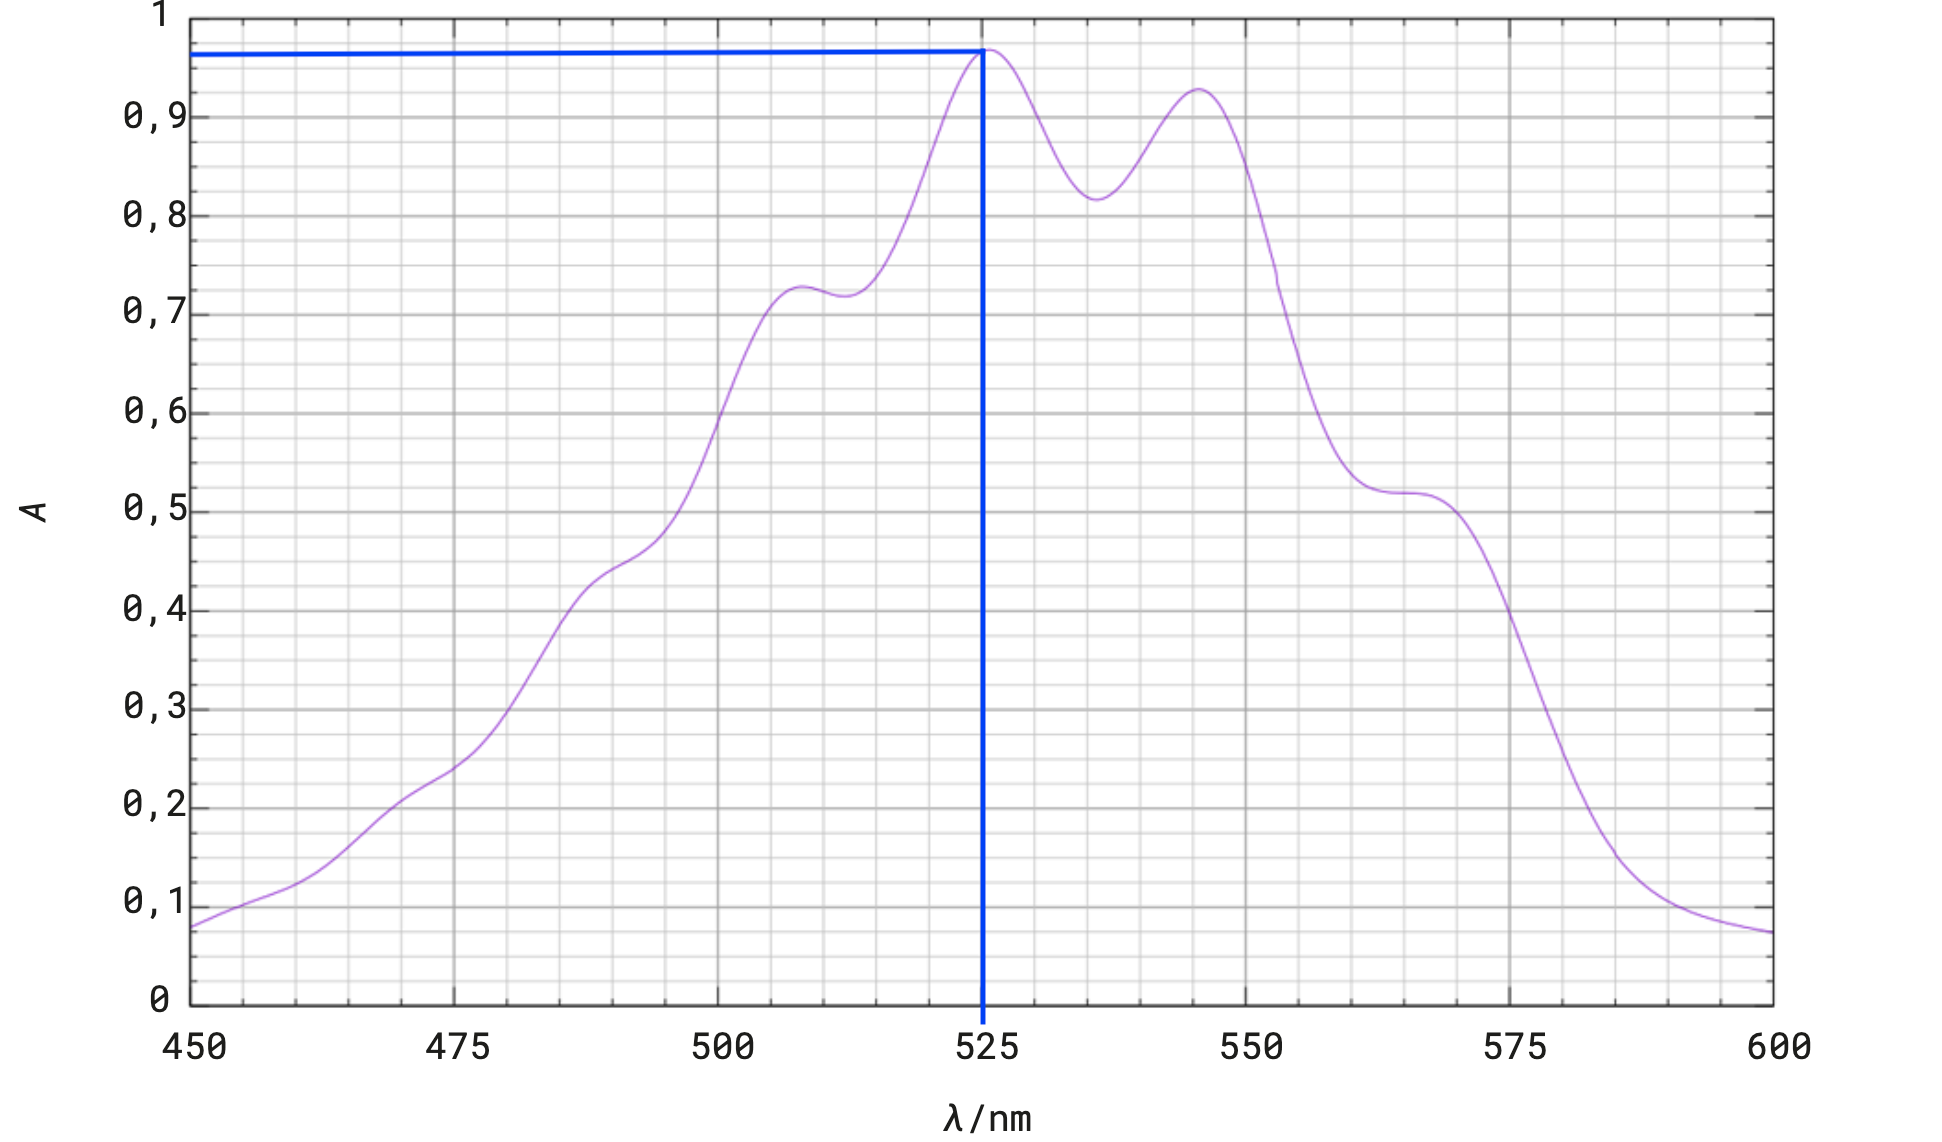
\includegraphics[width=\textwidth]{abs.png}
\end{center}
\caption{Aflæsning på absorptionsspektret}
  \label{fig:abs}
\end{figure}
\section*{Opgave 4 - Nonansyre}
\sol \\
\textbf{a.}
Det færdiggjorte reaktionsskema ses i \cref{fig:reak}.
\begin{figure}[H]
\begin{center}
  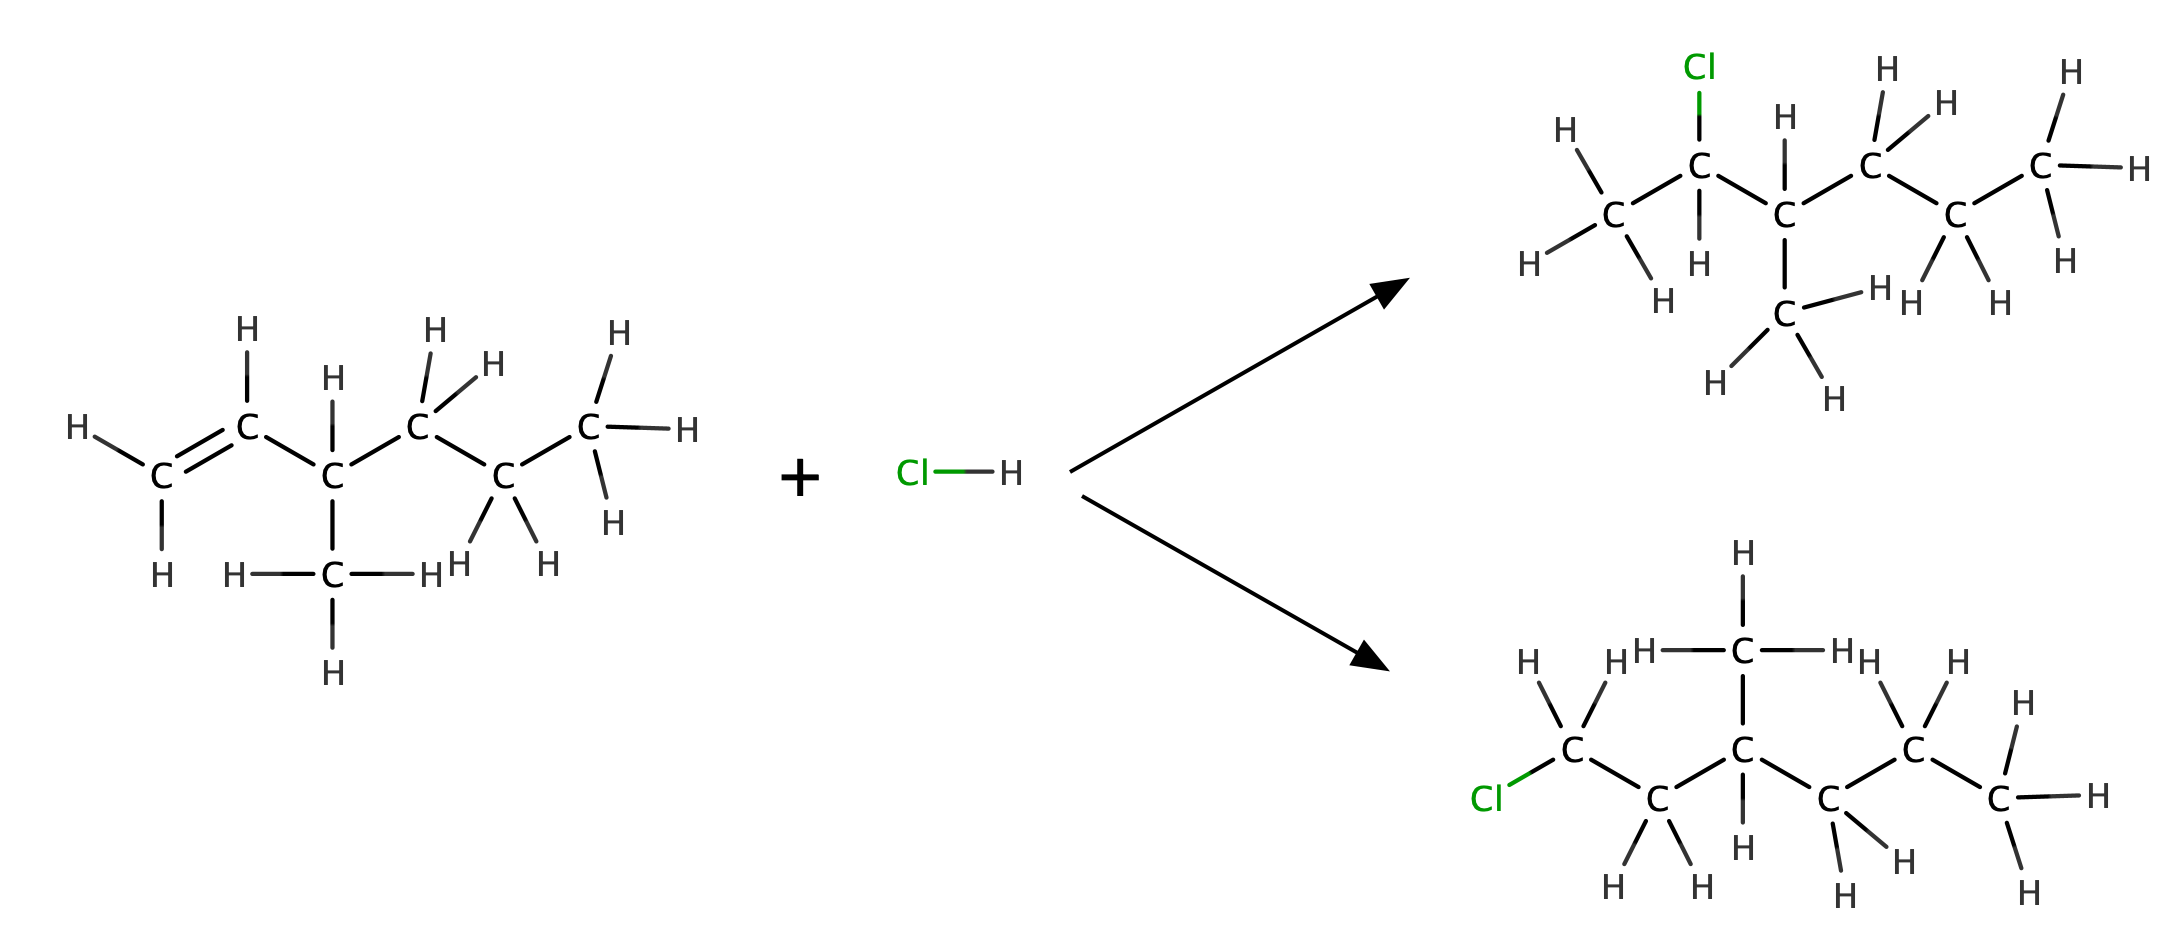
\includegraphics[width=\textwidth]{reak.png}
\end{center}
\caption{Reaktionsskema for første trin i fremstillingen af nonansyre}
\label{fig:reak}
\end{figure}
Siden stoffet spaltes under vandoptagelse, så er der da tale om en hydrolysereaktion. \\[1ex]
\textbf{b.}
Vi ser fra reaktionsskemaerne, at reaktionsforholdet mellem stof A og nonansyre er 1:1.
Der gælder da 
\begin{equation*}
\begin{split}
  n(\ce{A} )=n(\text{nonansyre} ) &\iff \frac{m(\ce{A} )}{M(\ce{A} )}=\frac{m(\text{nonansyre} )}{M(\text{nonansyre} )}\\
  &\iff m(\text{nonansyre} )=m(\ce{A} ) \cdot \frac{M(\text{nonansyre} )}{M(\ce{A} )}
\end{split}
\end{equation*}
Vi kan nu udregne det teoretiske udbytte af nonansyre.
\begin{equation*}
\begin{split}
  m_{\text{teo} }(\text{nonansyre} )&=m(\ce{A} ) \cdot \frac{M(\text{nonansyre} )}{M(\ce{A} )}\\
  &=12,9 \;\unit{g} \cdot \frac{158,24 \;\unit{g/mol} }{258,36 \;\unit{g/mol} }\\
  &=7,90098 \;\unit{g} 
\end{split}
\end{equation*}
Vi kan nu udregne, hvor stor det praktiske udbytte er ift. det teoretiske.
\begin{equation*}
\begin{split}
  \frac{m_{\text{prak} }(\text{nonansyre} )}{m_{\text{teo} }(\text{nonansyre} )}&=\frac{6,48 \;\unit{g} }{7,90098 \;\unit{g} }\\
  &\approx 0,820 \\
  &=82,0 \%
\end{split}
\end{equation*}
Udbyttet af nonansyre er altså $82,0 \%$ af det teoretisk mulige .
\\[1ex]
\textbf{c.}
Siden nonansyre og nonanoat er korresponderende syre-basepar, så gælder der, at 
\begin{equation*}
\begin{split}
  pK_b&=14,00-pK_s\\
  &=14,00+\log\left(\frac{K_s}{\;\unit{\textsc{m}}}\right) \\
  &=14,00 + \log\left(\frac{1,10 \cdot 10 ^{-5} \unit{\textsc{m}} }{\;\unit{\textsc{m}} }\right) \\
  &=9,04139
\end{split}
\end{equation*}
Der er altså tale om en svag base, og vi kan da udregne pH for opløsningen.
\begin{equation*}
\begin{split}
  \ce{pH} &=14,00 - \ce{pOH} \\
  &=14,00-\frac{1}{2} \cdot \left(pK_b-\log\left(\frac{c_b}{\unit{\textsc{m}} }\right) \right) \\
  &=14,00 - \frac{1}{2} \cdot \left(9,04139 - \log\left(\frac{0,109 \;\unit{\textsc{m}} }{\unit{\textsc{m}}}\right) \right) \\
  &\approx 9,00
\end{split}
\end{equation*}
Ved $25 \;\unit{\celsius} $ har den vandige opløsning af nonanoat altså $\ce{pH} = 9,00$. \\[1ex]
\textbf{d.}
I videoen afpipetteres $1000 \;\unit{\micro L} $ og fortyndes med demineraliseret vand. 
Blandingen titreres så med en $0,0940 \;\unit{\textsc{m}} $ opløsning af \ce{HCL}.
Titreringsreaktionen må være
\begin{equation}
\begin{split}
  \label{eq:tit}
\ce{C8H17COO-(aq) + H+(aq) -> C8H17COOH(aq) + H2O(l)} 
\end{split}
\end{equation}
Nonanoat og \ce{HCL} reagerer altså i stofmængdeforholdet 1:1.
Data fra titreringen sættes ind i logger pro, og en graf med $V(\ce{HCL})/\ce{mL}$ ud af $x$-aksen og pH op af $y$-aksen tegnes.
Det aflæses, at der ved ækvivalenspunktet er tilsat $12,5 \;\unit{mL} $ af \ce{HCl}-opløsningen hvilket ses i \cref{fig:tit}. 
\begin{figure}[H]
\begin{center}
  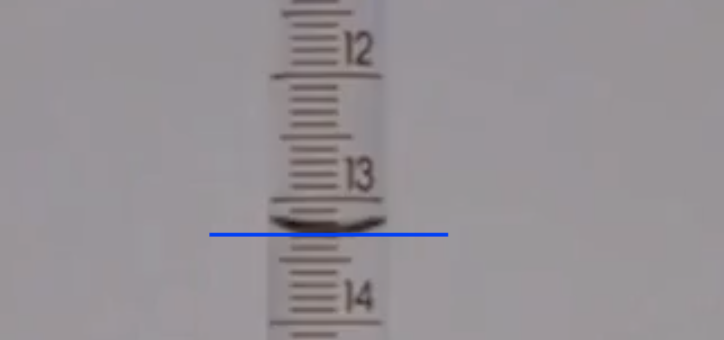
\includegraphics[width=\textwidth]{tit.png}
\end{center}
\caption{Ækvivalenspunktet aflæses på grafen i Logger Pro}
\label{fig:tit}
\end{figure}
Ved ækvivalenspunktet gælder der, at den tilsatte stofmængde af \ce{HCl} er lige med stofmængden af nonanoat:
\begin{equation*}
\begin{split}
  n(\text{nonanoat})&=n(\ce{HCl} )\\
  &=c(\ce{HCl} ) \cdot V(\ce{HCl} )\\
  &=0,0940 \;\unit{\textsc{m}} \cdot 12,5 \;\unit{mL} \\
  &=1,175 \;\unit{mmol} 
\end{split}
\end{equation*}
Ved fortyndingen af ukrudtsmidlet forbliver stofmængden af nonanoat den samme, og koncentrationen af nonanoat i ukrudtsmidlet må da være
\begin{equation*}
\begin{split}
  c(\text{nonanoat} )&=\frac{n(\text{nonanoat} )}{V}\\
  &=\frac{1,175 \;\unit{mmol} }{1000 \cdot 10 ^{-3} \;\unit{mL} }\\
  &=1,175 \;\unit{\textsc{m}} \\
  &\approx 1,18 \;\unit{\textsc{m}} 
\end{split}
\end{equation*}
For at bestemme den tilsvarende koncentration i g/L, beregnes først den molare masse for nonanoat.
\begin{equation*}
\begin{split}
  M(\text{nonanoat} )&=M(\text{nonansyre} ) - M(H)\\
  &= 158,24 \;\unit{g/mol} - 1,008 \;\unit{g/mol}\\
  &=157,232 \;\unit{g/mol} 
\end{split}
\end{equation*}
Koncentrationen af nonanoat i g/L betegner vi $k(\text{nonanoat} )$, og er 
\begin{equation*}
\begin{split}
  k(\text{nonanoat} )&=c(\text{nonanoat} ) \cdot M(\text{nonanoat} )\\
  &=1,175 \;\unit{\textsc{m}} \cdot 157,232 \;\unit{g/mol} \\
  &\approx 185 \;\unit{g/L} 
\end{split}
\end{equation*}
Dette er meget tæt på den deklarerede koncentration på $187 \;\unit{g/L} $, hvilket var, hvad vi skulle vise.

Vi har altså fået koncentrationen af nonanoat i ukrudtsmidlet til at være $1,18 \;\unit{\textsc{m}}  $, hvilket svarer til $185 \;\unit{g/mol} $.\\[1ex]
\textbf{e.}
Ved væske-væske ekstraktionen lades først nonanoat fra ukrudtsmidlet reagere med saltsyre for at omdanne nonanoat til nonansyre, som i reaktionsskemaet i ligning \ref{eq:tit}.
Siden nonansyre er så godt som uopløseligt i vand, så må den være upolær.
Heptan er også upolær og nonansyre kan altså opløses i heptan, hvilket saltsyren åbenlyst ikke kan.
Der dannes derfor to faser - én med nonansyre opløst i heptan og én med saltsyren og resten af ukrudtsmidlet.
Fasernes placering bestemmes af stoffernes densitet.

Fasen med nonansyre opløst i heptan tappes i en petriskål og lades stå indtil alt heptan er fordampet.
Massen af petriskålen vejes til at være $22,754 \;\unit{g} $ (\cref{fig:petri1}), og massen af petriskålen med nonansyren er $23,688 \;\unit{g} $ (\cref{fig:petri2}).
\begin{figure}[H]
\begin{center}
  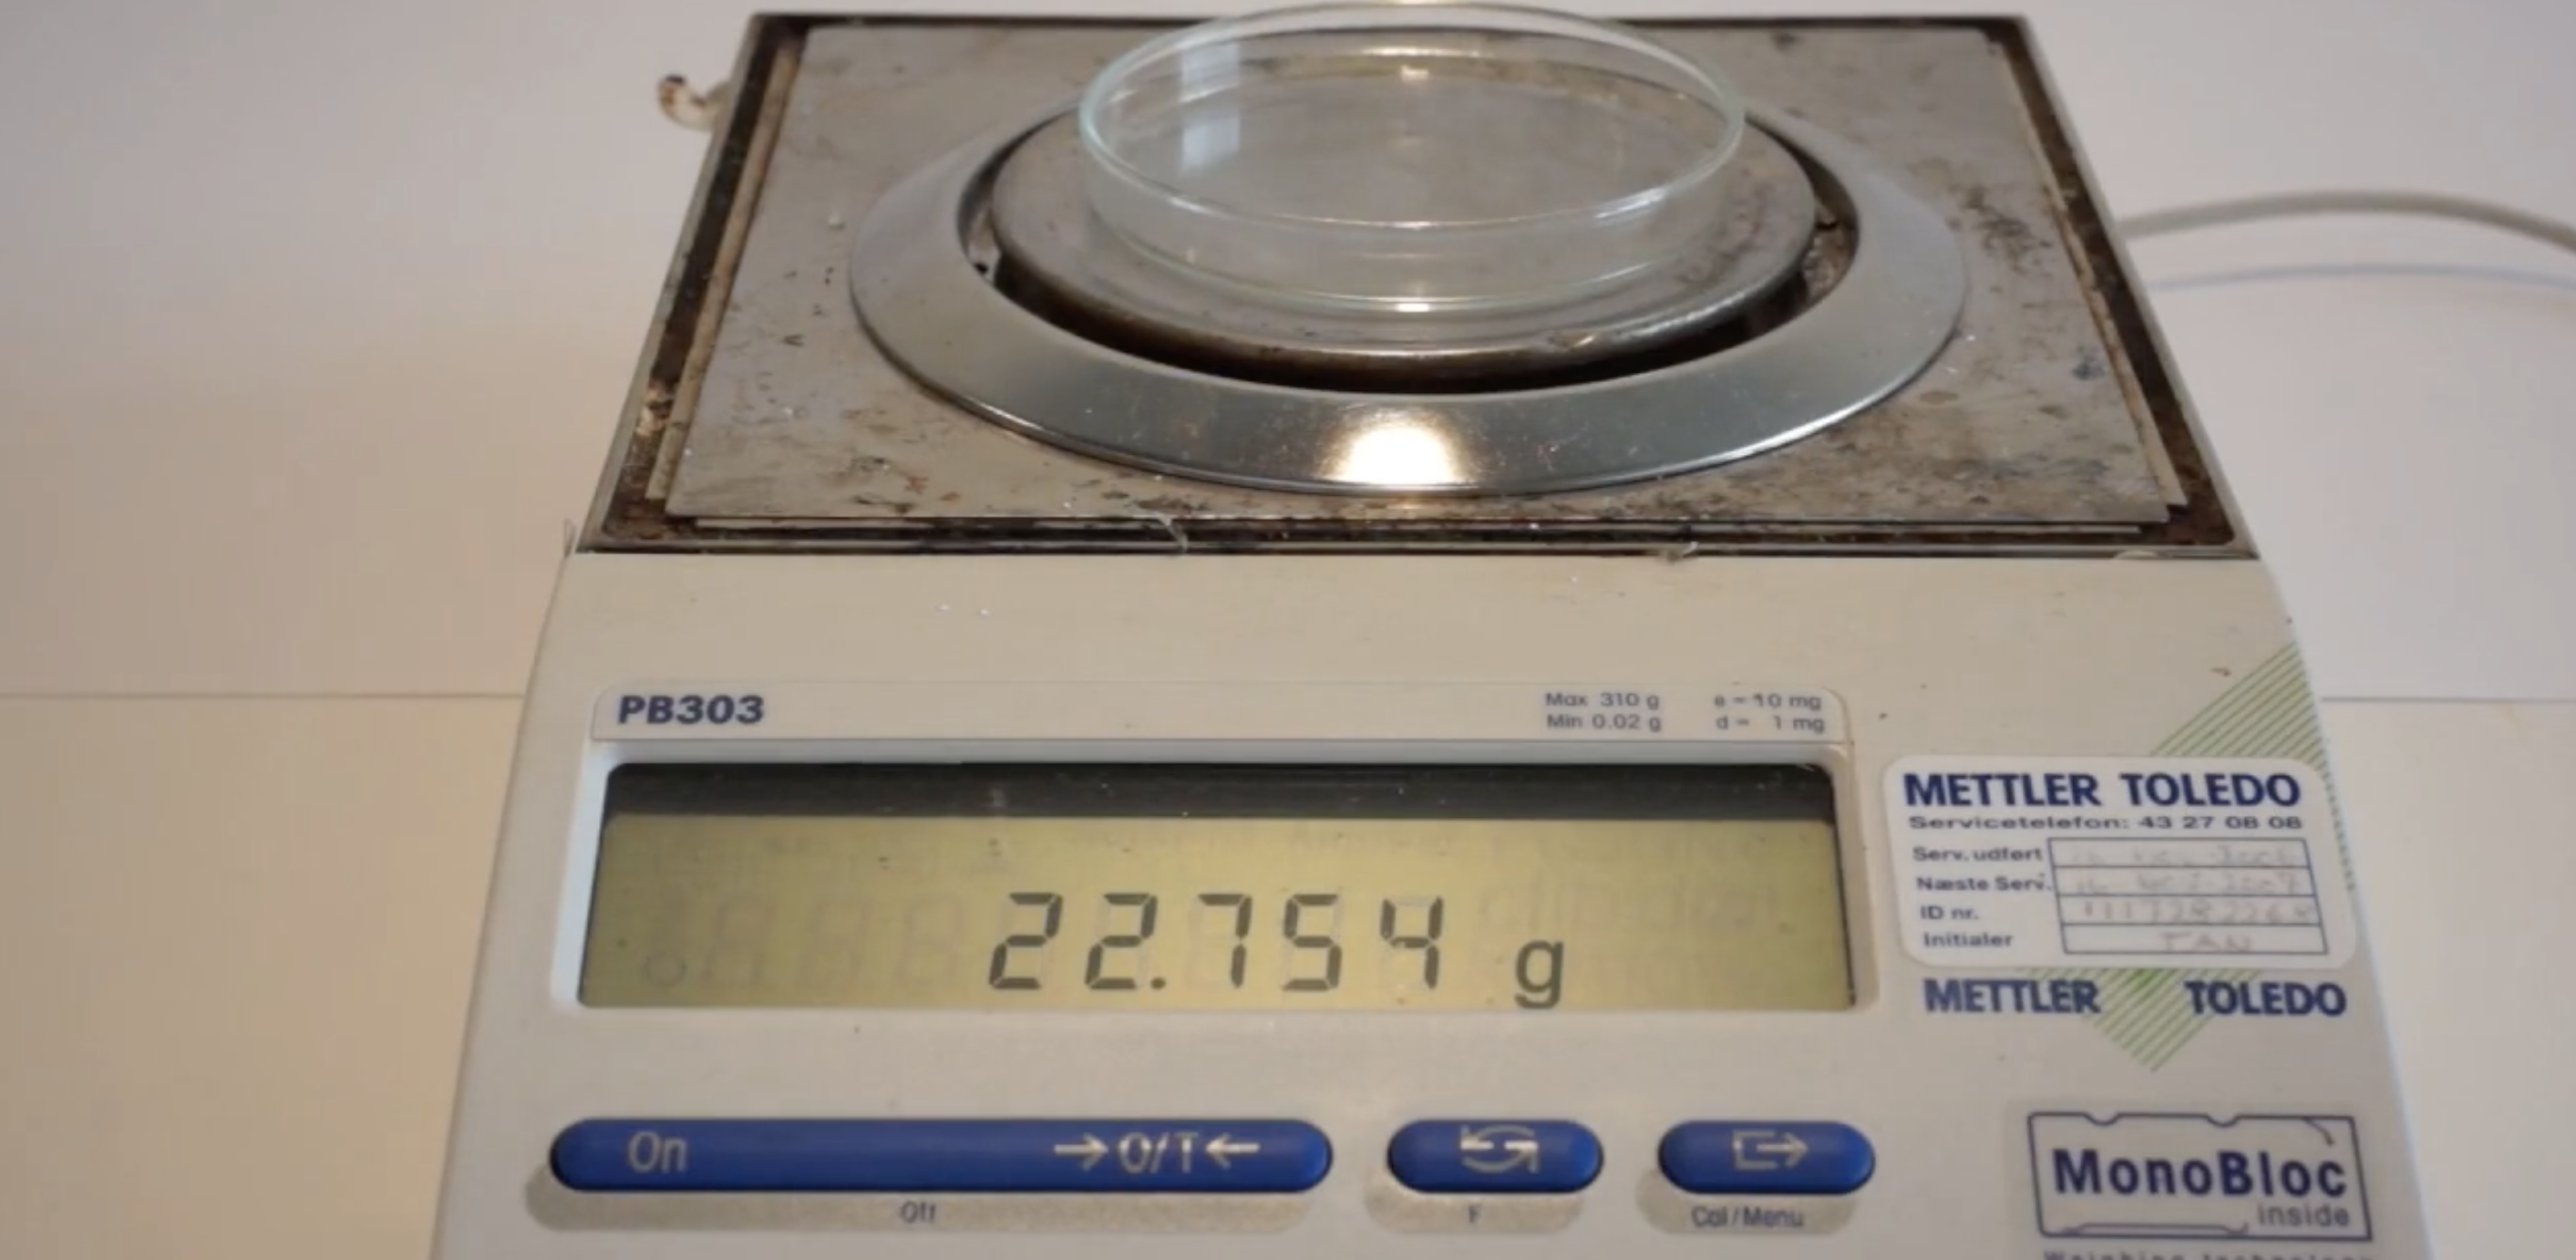
\includegraphics[width=\textwidth]{petri1.png}
\end{center}
\caption{Massen af den tomme petriskål bestemmes}
\label{fig:petri1}
\end{figure}
\begin{figure}[H]
\begin{center}
  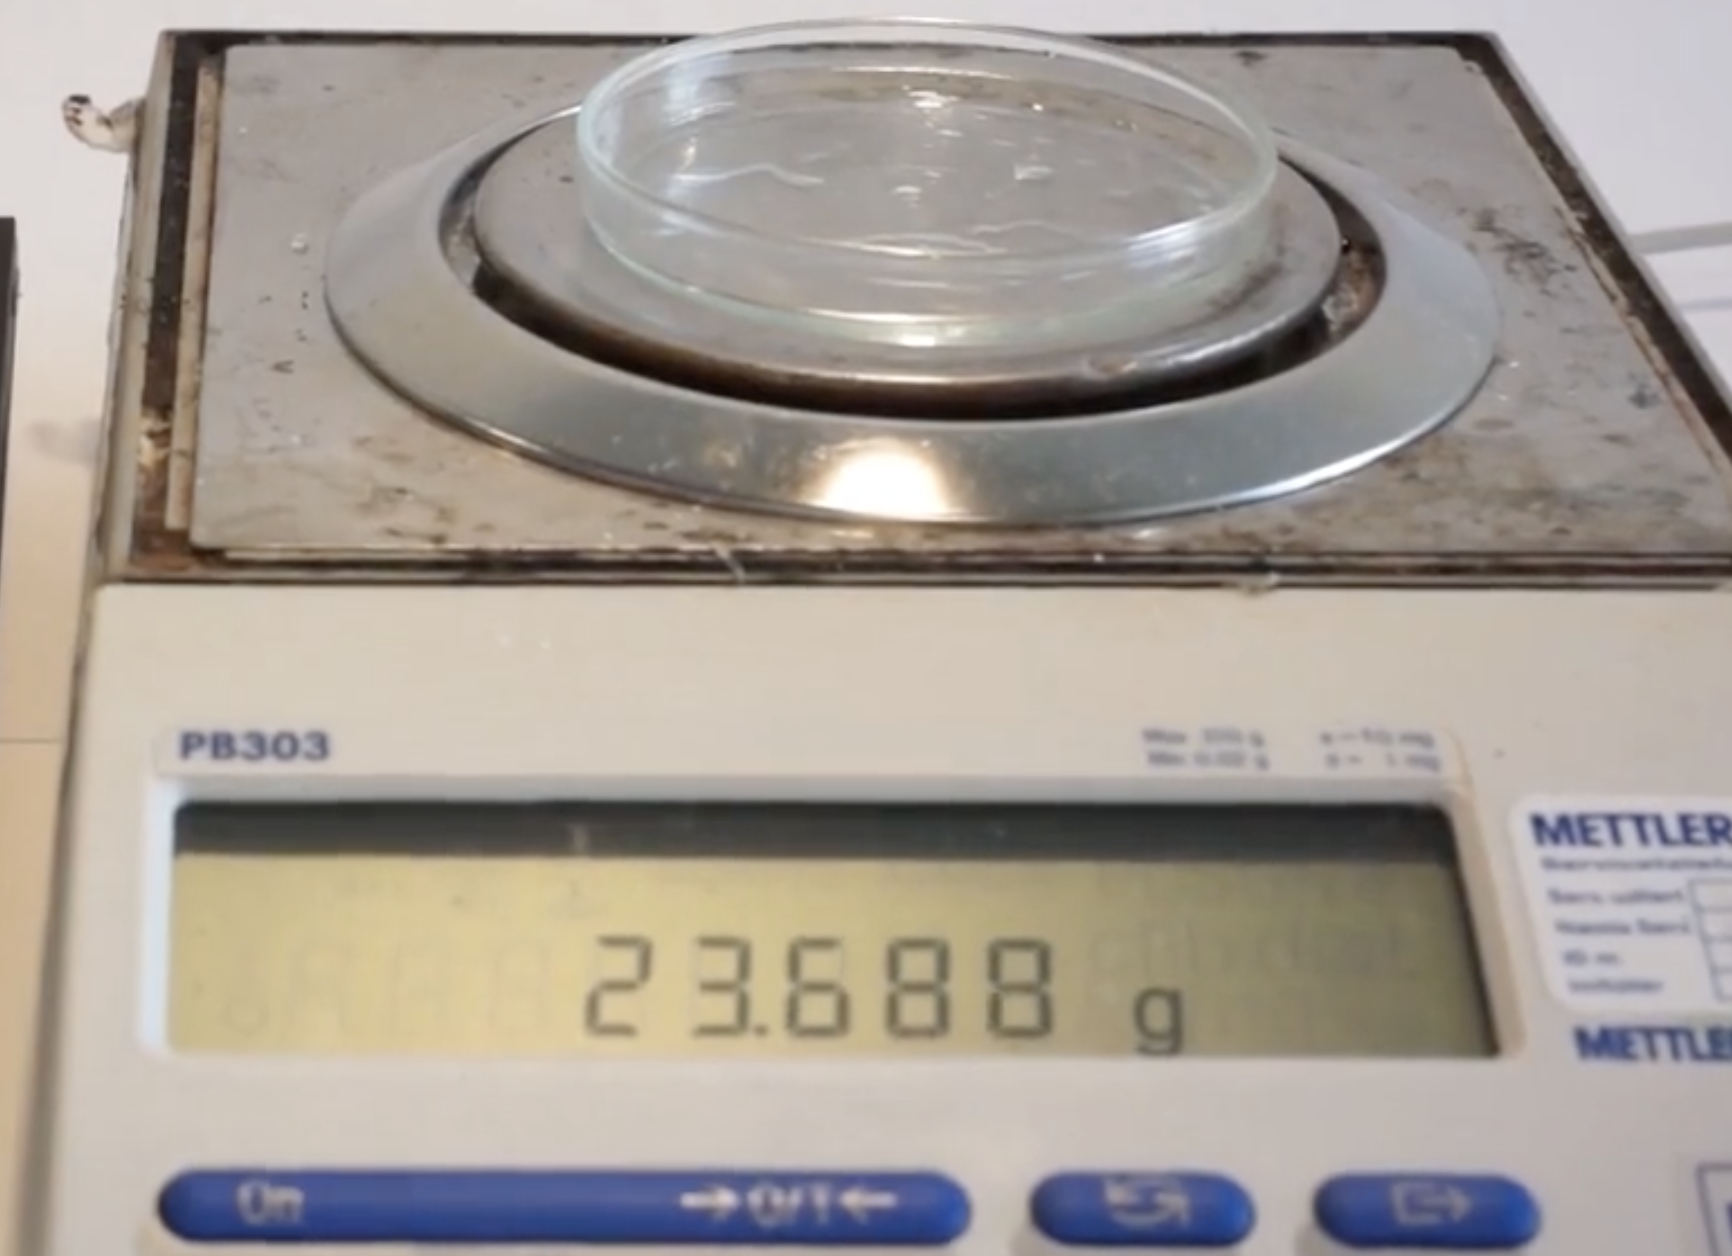
\includegraphics[width=0.6\textwidth]{petri2.png}
\end{center}
\caption{Massen af petriskålen med nonansyre bestemmes}
\label{fig:petri2}
\end{figure}
Massen af nonansyren er da
\begin{equation*}
\begin{split}
  m(\text{nonansyre} )&=m(\text{petriskål og nonansyre} ) - m(\text{petriskål} )\\
  &=23,688 \;\unit{g} - 22,754 \;\unit{g} \\
  &=0,934 \;\unit{g} 
\end{split}
\end{equation*}
Reaktionsforholdet mellem nonanoat og nonansyre i ligning \cref{eq:tit} er 1:1, og siden det er $5,00 \;\unit{mL} $ af ukrudtsmidlet vi har tilsat blandingen, så har vi 
\begin{equation*}
\begin{split}
  M_{\text{forsøg}}(\text{nonansyre} )&=\frac{m(\text{nonansyre} )}{n(\text{nonansyre} )}\\
  &=\frac{m(\text{nonansyre} )}{c(\text{nonanoat} ) \cdot V(\text{ukrudtsmiddel})}\\
  &=\frac{0,934 \;\unit{g} }{1,175 \;\unit{\textsc{m}} \cdot 5,00 \cdot 10 ^{-3} \;\unit{L} }\\
  &\approx 159 \;\unit{g/mol} 
\end{split}
\end{equation*}
Tabelværdien for den molare masse for nonansyre er 
\[
M _{\text{tabel} }(\text{nonansyre} ) =158,24 \;\unit{g/mol} 
\] 
Siden $M_{\text{forsøg}}(\text{nonansyre} ) \approx M_{\text{tabel}}(\text{nonansyre} )$, så kan det tyde på, at isolerede stof kan være nonansyre.

Vi vil nu undersøge det givne IR-spektrum.
En tabel over båndene ses i \cref{tab:IR}.
\begin{table}[H]
\centering
\begin{tabular}{@{}llllll@{}}
\toprule
  \makecell{Bånd\\nr.} & \makecell{$\frac{1}{\lambda }$/\unit{cm^{-1}}\\(aflæst)} & Intensitet & Bindingstilordning & Kommentarer & \makecell{$\frac{1}{\lambda }$/\unit{cm^{-1}}\\(tabel)}\\
\midrule
  1  & 1700 & Stærk & \ce{C=O} strækning & Carboxylsyre & 1695\\
  2 & 2850-2900 & Medium-svag & \makecell{\ce{C-H} strækning\\(C:$sp^3$)} & \makecell{ Alkyl\\(Flere bånd)} & 2810-2960 \\
  3 & 2500-3500 & Svag & \ce{O-H} strækning & \makecell{Caboxylsyre\\(Bredt bånd)} & 2500-3500\\
\bottomrule
\end{tabular}
\caption{Tilordning af absorptionsbånd i IR-spektret}
\label{tab:IR}
\end{table}
Bånd nr. 1 ved $1700 \;\unit{cm ^{-1}} $ kan skyldes \ce{C=O} strækningsvibrationer hos syregruppen. 
Det er i overensstemmelse med det svage brede bånd nr. 3, som så må skyldes \ce{O-H}-strækningsvibrationer.
Til sidst findes nogle bånd ved 2850-$2900 \;\unit{cm ^{-1}} $, som kan skyldes alkylkæden på nonansyre. 
Alle disse bånd (og manglen på andre bånd) kan tyde på, at det isolerede stof kan være nonansyre.
\section*{Opgave 4 - Husholdningssprit}
\sol \\
\textbf{a.}
Strukturen for 5-methylheptan-3-on ses i \cref{fig:5-methylheptan-3-on}.
\begin{figure}[H]
\begin{center}
  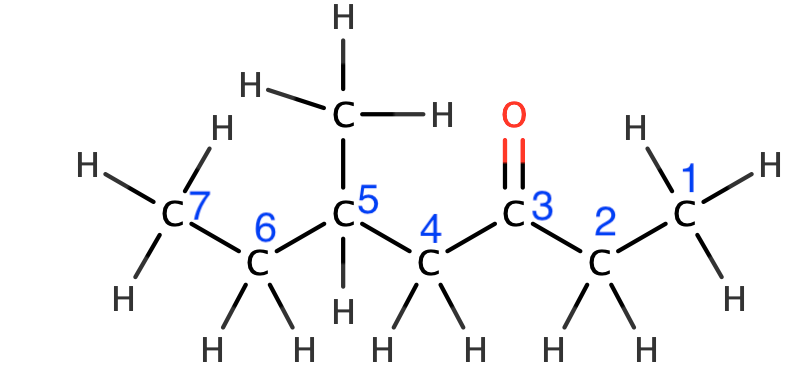
\includegraphics[width=\textwidth]{5-methylheptan-3-on.png}
\end{center}
\caption{Strukturformel for 5-methylheptan-3-on tegnet i MarvinSketch}
\label{fig:5-methylheptan-3-on}
\end{figure}
Da den funktionelle gruppe med højst prioritet er en oxogruppe, og det er i form af en keton, så må stoffets navn ende på -on.
Derudover tæller vi \ce{C}-atomerne fra den side af (se \cref{fig:5-methylheptan-3-on}), og oxogruppen sidder da på \ce{C}-atom nr. 3.
Det angives med et 3-tal før suffikset -on.

Den længste kæde af \ce{C}-atomer tælles til at være 7 lang, og heptan må derfor indgå i navnet.
Til sidst sidder der en methylgruppe på \ce{C}-atom nr. 5, hvilket giver præfikset 5-methyl-.

Stoffets navn bliver da 5-methylheptan-3-on.\\[1ex]
\textbf{b.}
En oversigt over resultaterne af de kemiske tests i videoen ses i \cref{tab:test}.
\begin{table}[H]
  \centering
  \begin{tabular}{@{}lll@{}}
  \toprule
  \thead{Destillat} & \thead{Reaktion med 2,4-dini-\\trophenylhydrazin} & \thead{Reaktion med Fehlings væske} \\
  \midrule
    P & Nej & Nej \\
    Q & Ja & Nej \\
  \bottomrule
  \end{tabular}
  \caption{Oversig over resultaterne af kemiske tests}
  \label{tab:test}
\end{table}
Vi ser som forventet, at P hverken reagerer med 2,4-dinitrophenylhydrazin eller Fehlings væske, da hverken vand eller ethanol indeholder nogen carbonylgruppe.

Vi ser også, at siden destillatet Q reagerer med 2,4-dinitrophenylhydrazin, så må det indeholde et stof med en carbonylforbindelse.
Altså må stof A og/eller B indholde en carbonylgruppe.

Da Fehlings væske som udgangspunkt reagerer med aldehyder men ikke ketoner, og Q ikke reagerer med Fehlings væske, så er det klart, at stof A og/eller B må være en keton.\\[1ex]
\textbf{c.}
Vi finder først den empiriske formel for stof A. 
I 100 g af stoffet er der
\begin{equation*}
\begin{split}
  n(\ce{C} )&=\frac{59,96 \;\unit{g} }{12,01 \;\unit{g/mol} }=4,9925 \;\unit{mol} \\
  n(\ce{H} )&=\frac{13,42 \;\unit{g} }{1,008 \;\unit{g/mol} }=13,3135 \;\unit{mol} \\
  n(\ce{O})&=\frac{26,62 \;\unit{g} }{16,00 \;\unit{g/mol} }=1,66375 \;\unit{mol} 
\end{split}
\end{equation*}
Stofmængdeforholdene beregnes:
\begin{equation*}
\begin{split}
  \frac{n(\ce{C} )}{n(\ce{O} )}&=\frac{4,9925 \;\unit{mol} }{1,66375 \;\unit{mol} }=3,0008 \approx 3\\
  \frac{n(\ce{H} )}{n(\ce{O} )}&=\frac{13,3135 \;\unit{mol} }{1,66375 \;\unit{mol} }=8,0021 \approx 8
\end{split}
\end{equation*}
Det fremgår da, at forholdet mellem stofmængderne af \ce{C}, \ce{H} og \ce{O} med stor nøjagtighed er 3:8:1.
Den empiriske formel for stof A er altså \ce{C3H8O}.
Siden der gælder at
\[
M(\ce{C3H8O} )=60,10 \;\unit{g/mol} \approx M(A)=60,095 \;\unit{g/mol} 
\] 
så må molekylformlen for A også være \ce{C3H8O}.
Vi ser nu på \ce{^1H}-NMR-spektret for A.
En opsummerende tabel ses i \cref{tab:HNMRA}.
\begin{table}[H]
\centering
\begin{tabular}{@{}lllllll@{}}
\toprule
  \makecell{Signal\\nr.} & \makecell{Kemisk skift\\(aflæst)\\$\delta$/ppm}& \makecell{Integral/areal\\(relativt antal ækvi-\\valente \ce{^1H}-atomer)}  & Opsplitning & Antal nabo-\ce{^1H}'er  & Tilordning & \makecell{Kemisk skift\\(tabel)\\$\delta$/ppm} \\
\midrule
  1 & 1,21 & 6 & Dublet & 1 & \ce{2C\textbf{H}3-CH-OH}  & 1,1\\
  2 & 2,17 & 1 & Singlet & 0 & \ce{-OH} & 0,5-5 \\
  3 & 4,05 & 1 & Septet & 6 & \ce{(CH3)2-C\textbf{H}-OH} & 3,9\\
\bottomrule
\end{tabular}
\caption{Tilordning af absorptionsbånd i \ce{^1H}-NMR-spektret for stof A}
\label{tab:HNMRA}
\end{table}
Der er tre signaler og dermed tre grupper af ækvivalente \ce{^1H}-kerner.
Fra signal nr. 2, der er en singlet ses det, at der må være tale om en alkohol.
Det er da klart fra arealet af signal nr. 1 og 3, at der må være 2 \ce{CH3}-grupper og én \ce{CH}-gruppe.
Fra opsplitningen ses det, at begge \ce{CH3}-grupper er bundet til en \ce{CH}-gruppe.
Siden der kun er én \ce{CH}-gruppe, så må de to \ce{CH3}-grupper altså være bundet til den samme \ce{CH}-gruppe.
Til sidst er der kun én mulighed ift. hvor \ce{OH}-gruppen kan side.
En strukturformel for A ses i \cref{fig:A}, hvor de \ce{^1H}-kerner, der svarer til hvert signal er numereret.
\begin{figure}[H]
\begin{center}
  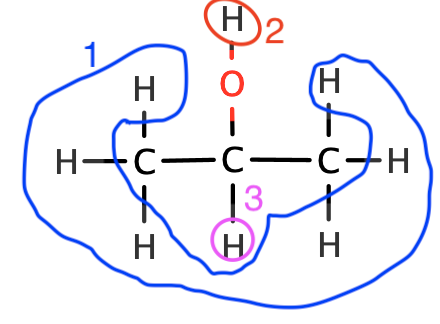
\includegraphics[width=0.7\textwidth]{A.png}
\end{center}
\caption{Strukturformel for A med \ce{^1H}-kerner numereret ift. tilsvarende signal}
\label{fig:A}
\end{figure}
Vi ser nu på \ce{^1H}-NMR-spektret for B.
En opsummerende tabel ses i \cref{tab:HNMRB}.
\begin{table}[H]
\centering
\begin{tabular}{@{}lllllll@{}}
\toprule
  \makecell{Signal\\nr.} & \makecell{Kemisk skift\\(aflæst)\\$\delta$/ppm}& \makecell{Integral/areal\\(relativt antal ækvi-\\valente \ce{^1H}-atomer)}  & Opsplitning & Antal nabo-\ce{^1H}'er  & Tilordning & \makecell{Kemisk skift\\(tabel)\\$\delta$/ppm} \\
\midrule
  1 & 1,05 & 3 & Triplet & 2 & \ce{ C\textbf{H}3-CH2-CO-CH3} & 1,1 \\
  2 & 2,11 & 3 & Singlet & 0 & \ce{C\textbf{H}3-CO-CH2} & 2,2 \\
  3 & 2,42 & 2 & Kvartet & 3 & \ce{CH3-C\textbf{H}2-CO-CH3} & 2,4\\
\bottomrule
\end{tabular}
\caption{Tilordning af absorptionsbånd i \ce{^1H}-NMR-spektret for stof B}
\label{tab:HNMRB}
\end{table}
Da stof A ikke er en keton, så må stof B være en keton (se delspørgsmål \textbf{b.}).
Fra opsplitningen fremgår det klart, at \ce{^1H}-kernerne hørende til signal 1 må koble til \ce{^1H}-kernerne hørende til signal 3.
Altså vil det sige, at der er en \ce{CH3}-gruppe bundet til en \ce{CH2}-gruppe.
Signal nr. 2 har areal på 3 og er en singlet.
Dens tilhørende \ce{^1H}-kerner  kobler altså ikke, og det må være på denne \ce{CH3}-gruppe, som carbonylgruppen \ce{CO} er bundet til. 
Der findes kun én struktur, der opfylder disse kriterier, og denne ses da i \cref{fig:B}, hvor de \ce{^1H}-kerner, der svarer til hvert signal er numereret.
\begin{figure}[H]
\begin{center}
  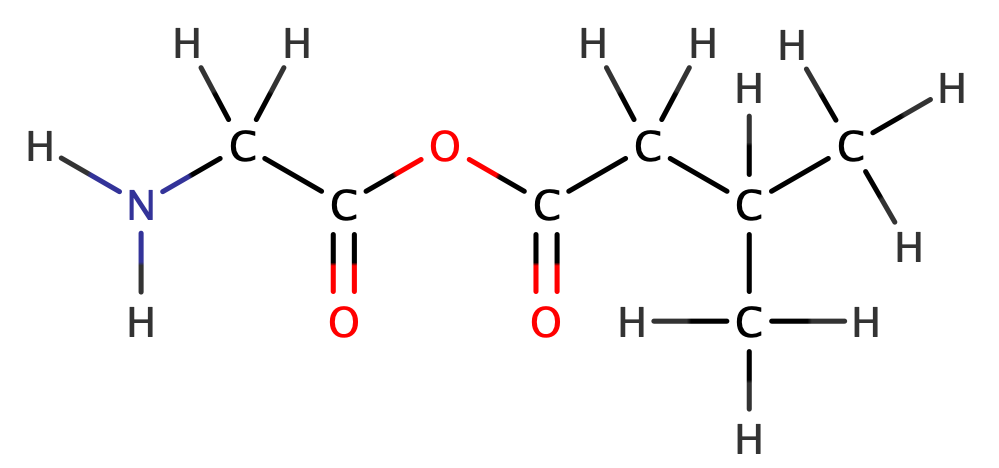
\includegraphics[width=0.7\textwidth]{B.png}
\end{center}
\caption{Strukturformel for B med \ce{^1H}-kerner numereret ift. tilsvarende signal}
\label{fig:B}
\end{figure}
For god ordens skyld kontrolleres resultatet ved at slå den molare masse for stoffet i \cref{fig:B}.
Denne fås til at være $72,11 \;\unit{g/mol} $, hvilket er i overensstemmelse med det oplyste for stof B.
\end{document}
